\chapter{Osciladores Senoidales}

\hspace{10pt}
El  circuito de la figura \ref{lab5_1} corresponde a un oscilador
Clapp:

Realizar los siguientes pasos:
\begin{enumerate}
	\item Calcular las resistencias de polarización de manera
	que $I_C\simeq 3mA$, estando la tensión del colector $V_C \simeq 6,5V$. Diseñar
	para que la caída de tensión en la resistencia de emisor sea aproximadamente el $5\%$ de la tensión de fuente.
	Verificar mediante las mediciones de continua correspondientes.
	\item  Calcular la red de realimentación para que la frecuencia de
	oscilación sea $f_o=200KHz$, teniendo en cuenta que $C_3=1nF$ ,
	$\frac{\displaystyle C_2}{\displaystyle C_1}=10$ (recordar que en un
	oscilador Clapp $C_3 \ll C_1$) , y $L_3$ es un inductor variable
	suministrado por la cátedra que permitirá el ajuste de frecuencia
	necesario. Para el cálculo teórico considere que el inductor tiene
	una $R_{serie}=0$.
	\item  Armar el circuito, ajustar $L_3$ para obtener
	$f_o=200KHz$ utilizando un osciloscopio. Medir la excursión de la tensión de
	salida $V_o$. Utilizando los dos canales del osciloscopio visualizar
	las tensiones de colector y base del transistor simultáneamente para
	calcular la ganancia de tensión. Sacar conclusiones respecto al
	resultado obtenido.
	\item Incrementar $C_2$ agregando capacidad en paralelo hasta
	que deje de oscilar, justificar.
	\item Retirar el inductor $L_3$ sin modificar su ajuste
	para efectuar con el Q-meter las mediciones de inductancia y Q
	correspondientes. Verificar que se cumplen las condiciones de
	oscilación.
	\item Construir un oscilador Pierce reemplazando
	$L_3$ y $C_3$ por un cristal de 4MHz provisto por la cátedra.
	Rediseñar los capacitores $C_1$ y $C_2$ adoptando un valor acorde a
	la nueva frecuencia de oscilación. Adoptar una relación
	$\frac{\displaystyle C_2}{\displaystyle C_1}\simeq 3$ para disminuir
	las exigencias de ganancia sobre el amplificador, tomar $C_1=56pF$.
	\item Realizar un informe escrito completo.
\end{enumerate}



\begin{figure}[h]
	\centering
	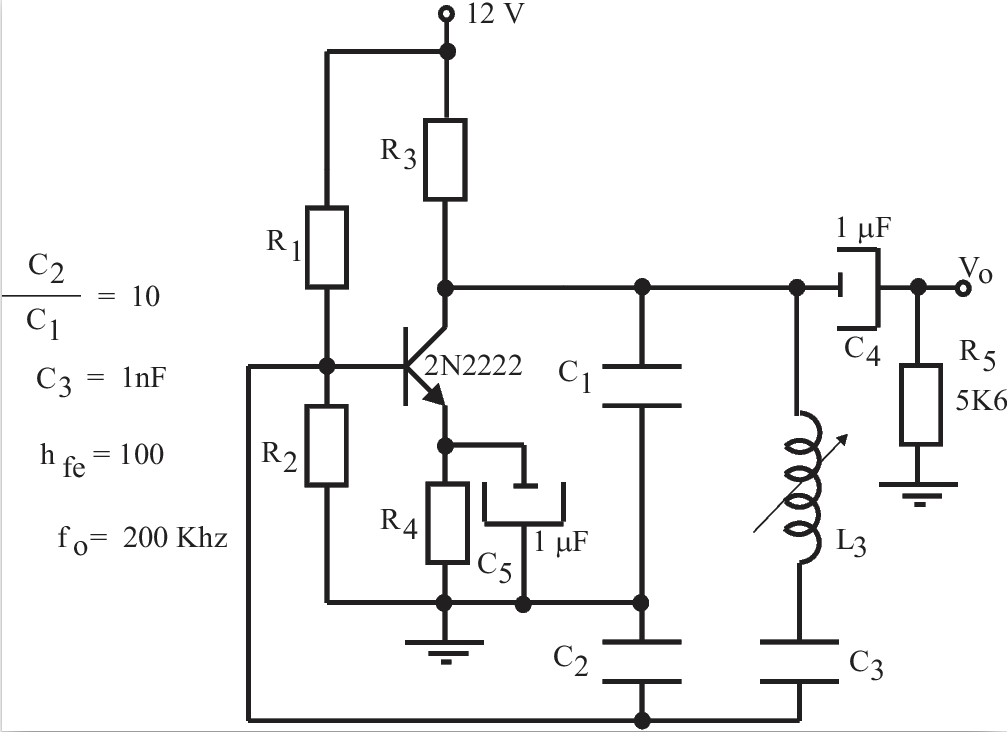
\includegraphics[width=0.8\linewidth]{figuras/lab5_1.png}\\
	\caption{}\label{lab5_1}
\end{figure}
